%%%%%%%%%%%%%%%%%%%%%%%%%%%%%%%%%%%%%%%%%%%%%%%%%%%%%%%%%%%%%%%%%%%%%%
% LaTeX Template: Project Titlepage
%
% Source: http://www.howtotex.com
% Date: April 2011
% 
% This is a title page template which be used for articles & reports.
% 
% Feel free to distribute this example, but please keep the referral
% to howtotex.com
% --------------------------------------------------------------------
% Preamble
% --------------------------------------------------------------------
\documentclass[paper=a4, fontsize=11pt,twoside]{scrartcl}	% KOMA

\usepackage[a4paper,pdftex]{geometry}	% A4paper margins
\setlength{\oddsidemargin}{5mm}			% Remove 'twosided' indentation
\setlength{\evensidemargin}{5mm}
\usepackage{pdfpages}
\usepackage[english]{babel}
\usepackage[protrusion=true,expansion=true]{microtype}	
\usepackage{amsmath,amsfonts,amsthm,amssymb}
\usepackage{graphicx}
\usepackage{blindtext}
\usepackage{enumitem}
\usepackage{longtable}
\graphicspath{{img/}}


% --------------------------------------------------------------------
% Definitions (do not change this)
% --------------------------------------------------------------------
\newcommand{\HRule}[1]{\rule{\linewidth}{#1}} 	% Horizontal rule

\makeatletter							% Title
\def\printtitle{%						
    {\centering \@title\par}}
\makeatother									

\makeatletter							% Author
\def\printauthor{%					
    {\centering \large \@author}}				
\makeatother							

\title{Logbooking Software for Science}

\author{
		F.P. van der Meulen, 500713781, (tel)+31 6 17506168\\
		Amsterdam, 2nd of March 2018\\	
		Amsterdam University of Applied Sciences\\
		HBO-ICT, Game Development\\
		C.J. Rijsenbrij\\	
		Software for Science\\
		Marten Teitsma\\
		February Semester, 2017-2018\\
}

			


\begin{document}
% ------------------------------------------------------------------------------
% Maketitle
% ------------------------------------------------------------------------------
\thispagestyle{empty}		% Remove page numbering on this page

%\printtitle
%\printauthor				% Print the author data as defined above

\maketitle


\newpage 
\printauthor

\newpage



\newpage
\tableofcontents

\newpage
\section{Preface}


\section{Abstraction}
The abstraction of the report.
\newpage
\section{Introduction}
This is a student thesis from the Amsterdam University of Applied Sciences from the HBO-ICT-Game Development study course. This student thesis is made for the organization Software for Sciences. \\
Software for Science is an organization, at the moment lead by Dr. Marten Teitsma, that combines software with science. The organization works with Astron, eScience center and CERN to create software for their scientific experiments. \\
Conseil Européen pour la Recherche Nucléaire, CERN, is a science research center in Geneve, focused on researching nuclear energy. This happends mostly with particle research, eg, shooting particles against each other in order to find out what energy comes free from one of those runs. CERN achieves this with the help of particle colliders. One of those particle colliders is ALICE. \\
ALICE, A Large Ion Collider Experiment, has its own bookkeeping system. This system makes sure that the runs ALICE makes are recorded into the bookkeeping system so that researchers, collaborators and other people can look back upon the runs.  \\
At the moment, ALICE is under maintenance. During the maintenance, subsystems and parts of ALICE are being renewed. Before the maintenance started, the request for a new bookkeeping system was made. There are three reasons for a new bookkeeping system. The first reason is that the new system must combine the bookeeping system with AliMonitor, a monitoring system. The second reason is that there are multiple desired functions that are not added to the current system, such as automated report making with the help of a template(at the moment, the shifter that has to make a report copies the previous report(bron interview transcriptie). The third reason is that most of the technologies and frameworks used to develop the system is outdated due to the fact that development started around 2009. From 2009 untill now, new featues were added to the system and new tables were created in the database. This caused that the structure of the code is not organized, the database structure was not efficient in handling requests from the client. \\
Software for Science is planning to deliver the new bookkeeping system in January. At first, they plan to show a prototype of the bookkeeping system in June to CERN workers that are involved with the creation of the prototype. After the protoype, Software for Science hosts a summer school in which interested people can work on expanding the protoype and start on creating new features. Finally, at September of 2018, a semsester at the University of Applied Sciences will be held in order to create the final product. \\
Due to the size of the project, the little amount of time avaliable for the development, and the many whishes from CERN, 
considerations for the prototype must be made. This brings the following main research question: \\ \\
Which requirements can be implemented into the logbook system for ALICE?
\\ \\
In order to make a prototype for the new bookeeping system, the back-end and the front-end are seperated from each other. This was done due to the fact that the scope of the project would become to big. Another reason was that the front-end and back-end of the application will run differently. While the back-end will run on a server, the front-end must run on every computer at CERN. This thesis handles the back-end of the new logbooking system. The front-end will be developed by Naomi Nazar. 
\\ 
This thesis is split into four parts. Every part resembles a sub research question. An explanation why these sub research questions are importand and how they could help solving the main research question can be found later in the thesis. The sub research questions are as followed: \\
\begin{enumerate}
\item What database would fit the prototype?
\item Which requirements are important for the logbook system for ALICE?
\item What are the consequences for the development process of the prototype based upon the important requirements and the database choices?
\item How can the prototype be developed?
\end{enumerate}
 

 

\newpage
\section{Techniques}
This chapter will talk about the techniques used to create the prototype.

\subsection{Javascript}
The main programming language for this research is Javascript. Javascript was one of the hard requirements set by CERN.

\subsection{AliceO2/WebUi framework}
The preference of CERN is to use CERN's own developed frameworks as much as it is possible to do so. The WebUi framework is a framework to handle HTTP requests made by the client, in this case, the front-end. The base of this framework is the ExpressJs framework. \\
The ExpressJs framework is a lightweight framework for handling HTTP calls. CERN has expanded this framework with features such as Json Web token support, debug logger systems and support for CERN's own authentication system,

\subsection{Postgresql}
The main database that will be used for the prototype is a Postgres database. 

\subsection{Mocha}
The testing framework that has been chosen is the Mocha testing framework.

\subsection{Sublime text 3}
The development enviroment for developing the prototype is Sublime Text 3.

\subsection{Lucichart}
Lucichart is used for the creation of the Enitity Relation Diagram's and the Unified Moddeling Language Diagrams.

\subsection{Scrum}
Scrum is the 

\newpage


\section{Methods}
This chapter discusses the methods used to solve the research questions. The four research questions that were earlier created will be discussed. 

\subsection{Database}
In this section, different kinds of databases will be compared with each other in order to find out which database would be the best choice for the logbook prototype. \\
The REST-API will make use of the SAMS authentication API created by CERN. However, this API is not made availiable yet for the back-end of the bookkeeping system prototyp. To still being able to work with users, the database scheme(bron) technique will be used. With the help of this technique, the database can be 'split' into two different databases. This will not affect the later implementation of the SAMS API.
What is also important, is the design of the database. The database design will be created with the help of an Enitity Relation Diagram(bron). This diagram displays all the entities that are in the database and shows the relation between different entities. Due to 'splitting' the database, two different ERD's will be shown. \\
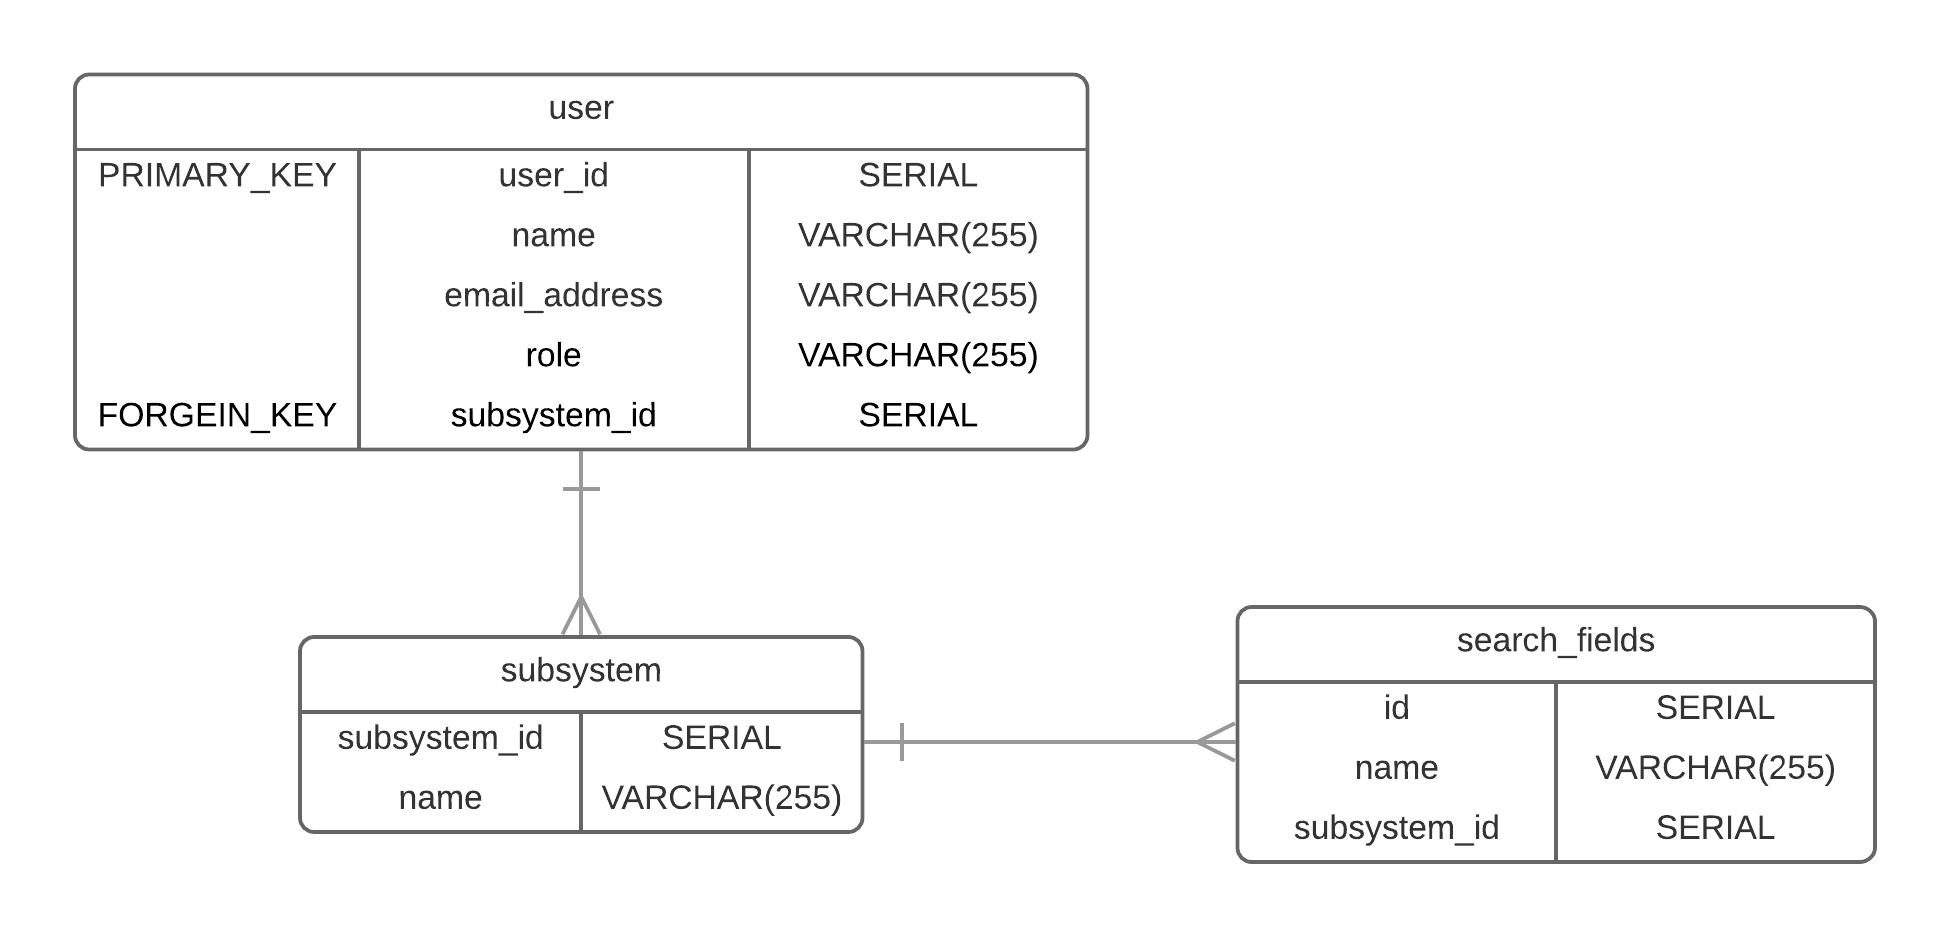
\includegraphics[scale=1]{ERDUser}

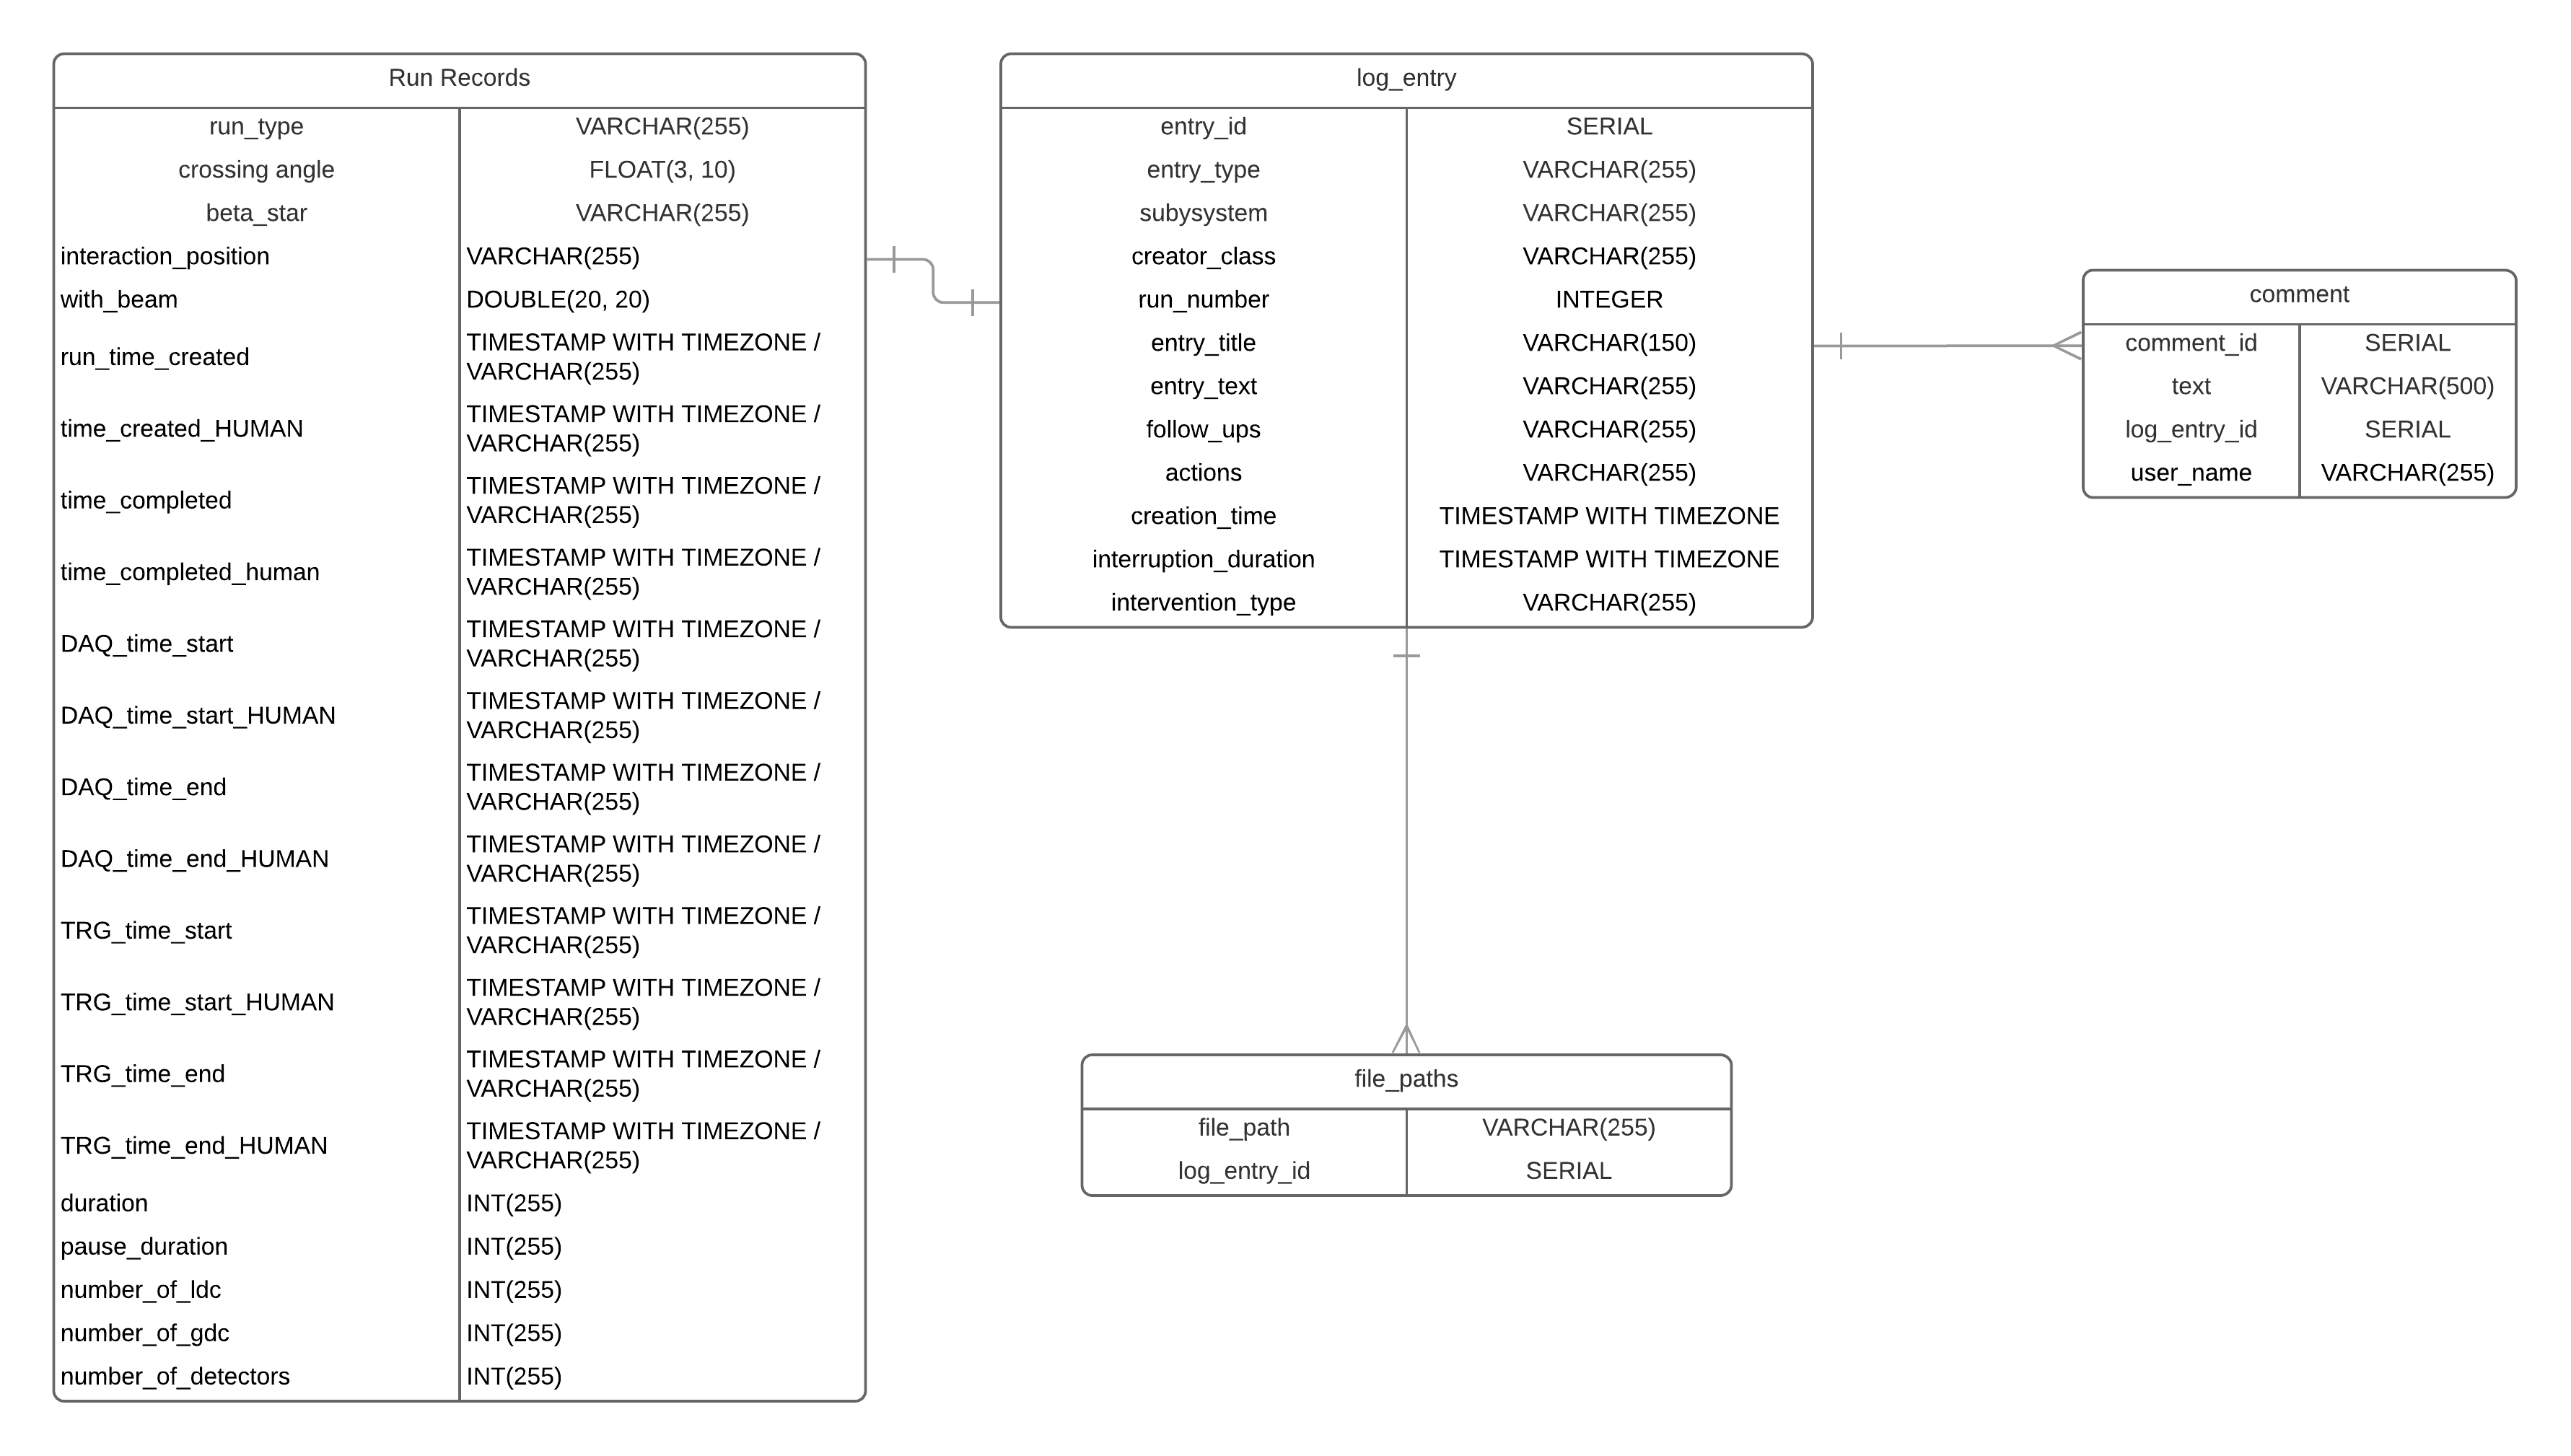
\includegraphics[scale=0.5]{ERDLogEntry}

The main cirteria for choosing the database is that the database needs to be open-source. Since the logbooking prototype is open-source, using a database that isn't open-source would make the prototype not open-source anymore. To find out which database is the best for the prototype, tests will be made to test the different kind of databases. \\
The results of the test can be found below: \\

Tabel met de resultaten \\



\newpage
\subsection{Req analysis}
This section of the thesis will discuss the requirements analysis. There are over 120 requirements created by CERN. It is impossible to use every requirement in the prototype, due to scale of the requirements and due to time constraints that are set. An analysis is needed in order to check which requirements are nescessary to add to the protoype and which requirements can be left out.  \\
Inside the requirement document were some vague terms that weren't explained. The terms were follow-ups, on call intervention, announcements, and an EOS report. Iets over de features die er staan, maar onduidelijk zijn. \\
To solve the vague requirements and unknown wishes, a former shifter by the name of Pascal Buschoten has been interviewed. The full transscript can be found in the attachments. The interview with Pascal clarified a couple of terms like the on call intervention and the end of shift reports with templates. On call Interventions are emergency issues with a detector, a particle collider or anoter system that need to be solved as soon as possible. These issues need to be fixed within a very short amount of time. Currently, there is not a formal template availiable for the EOS reports  and because of that, all the reports do not follow the same structure. With a template, it is better to evaluate all the EOS reports).\\
A criteria for the prototype was given by Dr. Teitsma. This criteria was that all the requirements related to the Subsystem Run Coördinator must be added to the prototype. This criteria was crucial for the requirement analysis. \\
During a meeting at the ninth of may, one of the developers from CERN, Vasco Chibante Barroso, stated that he preferes that the prototype would focus more on the features instead of the roles and the authentication. This complicates the planning of the new features for the prototype. Therefore, there will be a focus on both the features wish from CERN and a focus on the SubSystem Run Coordinator from Dr. Teitsma. \\ 
The technique that will be used is the Analytic Hierarchy Process technique.(bron van pakistaanse artikel die dit voor het eerst beschrijft). "In AHP, initially whole requirements are recognized and then criteria under which these requirements will be preferred. In AHP we pair wise analyzing  between  the  probable  pairs  of  the  hierarchy. 
Now users can recognize the possible relationship between 
the hierarchies. We then pair wise analyze them and users can select its preferences from the scale which ranges from 
1 to 9."(Javed Ali Khan, Izaz Ur Rehman, Yawar Hayat Khan, Iftikhar Javed Khan, Salman Rash, 2015). One of the main advantages of using this technique is that ""(Bron pakistaanse artikel). The second software requirements analysis technique that will be used for the software is the Hierachy Analytic Hierachy Process technique(bron van artikel die dit voor het eerst beschrijft). HAHP is a technique that creates so called planes of requirements in order to simplify the requirement analysis process. A plane is a group of requirements that are grouped together if they share a similarity. These planes can, for example, align to a user of the system or a feature that will be implemented into the final product. For this requirement analysis, the planes will consists of features since this will be more important for the prototype than the users themselfs. \\
Lastly, time will be an important factor for the requirement analysis. The time will be estimated using the story points technique. This technique consists of giving  points to requirements in order to organize the effort and scale of a requirement. The range of these points are:  zero, zero point five, one, two, three, five, eight, thirteen, 20, 40 and 100. \\ \\
Applying the chosen techniques to the requirements document results in tables with pioritized requirements with scrum points given to the requirements. The requirements are grouped by feature so that it is easier to read. There were numerous requirements that were double. In cases like these, the requirements were the same, but, the requirements were assigned to different roles. These requirements are grouped together to prevent duplicity. \\
The four most important features will be given and explained due to the amount of requirements. The complete requirements table can be found as an attachment.\\

\subsubsection{Entries}
These requirements are about the different kind of entries into the system(log entries, on call interventions, run entries etc.). This feature sits at the core of the to be delivered product and therefore has the most requirements attached to it. Due to the amount of requirements that are related to the entries, this section is divided into different sections for readibility. 

\begin{longtable}{ | p{3cm} | p{8cm} | p{1.5cm} | l |}
\hline
Role & User Story & Piority & Time \\ \hline
Shifter &  A shifter makes an entry into the database consisting of several items. Each entry records the following items: time of creation,which class the creator originates: human, type of entry, general, EOS, DCS, number of run, author of the entry, title of the entry, log entry, follow ups, files and actions & 9 & 8 \\ \hline
User & As a user, I want to search log entries by different criteria (e.g. title, content, author, creation date,(...) and have the results listed. & 9 & 8 \\ \hline
Run coördinator, SRC, STC and Shifter& As run coördinator, SRC, STC or as Shifter, I may need to attach files to log entries. These files may contain text or binary information (PNGs, JPGs etc...) (Roberto Divia). & 8 & 8 \\ \hline
Subsystem expert & As a subsystem expert, I want to attach quality flags to runs so that
physicists can use them while searching for good data sets for their analysis (Vasco Chibante Barroso). & 8 & 8 \\ \hline
\end{longtable}


\subsubsection{Reports}
A requested feature in the new final product was the automatic creation of reports and templates. This is not availiable in the current product, therefore, there are a couple of requirements referencing towards the creation of templates and reports.
\begin{longtable}{ | p{2cm} | p{8cm} | p{1.5cm} | l |}
\hline
Role & User Story & Piority & Time \\ \hline
Subsystem Run Coördinator & As a SRC I would like to be able to create my own detector specific templates for example On-Call interventions. In this case I can specify the relevant information which are required from the OnCall shifter for different kind of “standard” events (Robert Munzer). & 8 & 20 \\ \hline
Shifter &  As a shifter, I want to have templates that prefill most of my end-of-shift reports from the available metadata so that I don’t need to fill inmyself what the system already knows (Vasco Chibante Barroso). & 2 & 13 \\ \hline
\end{longtable}

\subsubsection{Email}
Sending emails is availiable in the current system, however, the current way the emails are send are send in a spam related way, eg, a shifter receives an email if another shifter makes an entry from another subsystem. Therefore, the email system needs to be optimized and it should be designed in a way that will not be annoying to the user. The reason that this is of more importance, is that it is easy to adjust the way the emails are send, how the emails look like and who receives an email. Therefore, with adding it to the prototype, it will be easier to adjust it to the wishes of the users.
\begin{longtable}{ | p{2cm} | p{8cm} | p{1.5cm} | l |}
\hline
Role & User Story & Piority & Time \\ \hline
ALICE member & As an ALICE member, I would like to receive via email a global summary of each LHC Fill in order to follow ALICE operations without visiting the bookkeeping tools. Currently in the ALICE logbook, I like that I receive via email a document with info on efficiency and EOR Reasons and that on the body of the email there is a summary for
each fill (Vasco Chibante Barroso). & 8 & 20 \\ \hline
Subsystem Run Coördinator &  As a subsystem responsible, I want to be notified by email (or other
channels) of log entries which are related with my subsystem so that I can better follow-up activities without having to constantly visit the product, e.g. EOS report (Robert Munzer) (Vasco Chibante Barroso). & 8 & 13 \\ \hline
Run coördinator & As run coördinator I may request to receive automatic e-mails concerning all Logbook entries that include all systems (either without distinction or using special selection criterias). The e-mail delivery address will probably be an e-group (single e-mail address <...>@cern.ch)(Roberto Divia). & 6 & 13 \\ \hline
\end{longtable}

%\subsubsection{\ref{table:hans}}
\subsubsection{Roles and Authentication}
There are different kinds of roles and users in the bookkeeping system. It is possible that a user is assigned to multiple subsystems with different roles. Only certain roles can move in and out of subsystems. Since the different roles play an important part in the bookkeeping system, it is mandatory to have them in the prototype.

\begin{longtable}{ | p{2cm} | p{8cm} | p{1.5cm} | l |}
\hline
Role & User Story & Piority & Time \\ \hline
User & As a user, I want to be able to login with my CERN credentials to avoid having to remember a new set of credentials. This should be done by using the CERN authentication method. & 9 & 13 \\ \hline
Run coördinator, SRC and Administrator &  As run coördinator, SRC or Admin, I must be able to move collaborators to and out of subsystem teams. These action may be conflict the information stored in SAMS (Roberto Divia). & 9 & 13 \\ \hline
Run coördinator and SRC &  As run coördinator or SRC I need to give ALICE collaborators write or read-only access to the logbook. These rights will be superseeded by equivalent rights given according to the function of the user (e.g. a ALICE collaborator with read-only access will be given write access during the time of his/her duties as a shifter, subsystem run coördinator or system team member) (Roberto Divia).&6&13 \\ \hline

\label{table:hans}
\end{longtable}



\newpage
\subsection{Consequences}
This section of the thesis will be about the consequences for the development of the prototype after the pioritization of the requirements and the database choice. The wishes of the front-end(being developed by Naomi Nazar) will be taken in account aswell, due to the reason that Naomi has to decide what she wants to show for the prototype on the front-end side. \\
To help the development of the prototype, agile techniques will be used in order to plan and organize the development process. The technique that will be used for the development of the prototype will be the SCRUM(bron) technique. At the pioritization of the requirements, a time measuerment was given. The time measurement was important, because with the times estimated, it will be possible to create sprints. A sprint is a set time in which a development team works to fullfil the requirements. The length of a sprint varies from one day till two weeks. The recommended length for a sprint is one week, therefore, this lenght will be chosen. Every requirement that was estimated had a time measuerment in story points given. The amount of story points a developer can work on in a week varies. Since the story points are estimated, it will be hard to say how much story points a developer can take in a week. For the prototype, a maximun of 40 story points per sprints will be chosen. \\
The front-end and the back-end were asked to come up with features that they think should be added to the prototype. Both the front-end and the back-end used the pioritzed requirements as a start, then looked at the amount of time needed to complete the requirements. These are the requirements that have chosen to be added to the prototype. \\
\begin{longtable}{ | p{2cm} | p{8cm} | p{1.5cm} | l |}
\hline
Role & User Story & Piority & Time \\ \hline
Run coördinator, SRC, STC and Shifter& As run coördinator, SRC, STC or as Shifter, I may need to attach files to log entries. These files may contain text or binary information (PNGs, JPGs etc...) (Roberto Divia). & 8 & 8 \\ \hline
Shifter &  As a shifter, I want to have templates that prefill most of my end-of-shift reports from the available metadata so that I don’t need to fill inmyself what the system already knows (Vasco Chibante Barroso). & 2 & 13 \\ \hline
Subsystem expert & As a subsystem expert, I want to attach quality flags to runs so that
physicists can use them while searching for good data sets for their analysis (Vasco Chibante Barroso). & 8 & 8 \\ \hline
User & As a user, I want to search log entries by different criteria (e.g. title, content, author, creation date,(...) and have the results listed. & 9 & 8 \\ \hline
Run coördinator &  As run coördinator, I want to attach tags to runs so that I can then use them while searching (Vasco Chibante Barroso). & 4 & 8 \\ \hline
User &  As a user, I want to list all runs that match a given criteria to create my own run set. & 8 & 8 \\ \hline
Subsystem Run Coördinator &  As a subsystem responsible, I want to be notified by email (or other
channels) of log entries which are related with my subsystem so that I can better follow-up activities without having to constantly visit the product, e.g. EOS report (Robert Munzer) (Vasco Chibante Barroso). & 8 & 13 \\ \hline
SRC & As subsystem run coördinator I may request to receive automatic emails concerning all Logbook entries that include the System I am working for (either without distinction or using special selection criterias). The e-mail delivery address will probably be an e-group (single e-mail address <...>@cern.ch) (Roberto Divia). & 8 & 13 \\ \hline
Run coördinator, SRC and Administrator &  As run coördinator, SRC or Admin, I must be able to move collaborators to and out of subsystem teams. These action may be conflict the information stored in SAMS (Roberto Divia). & 9 & 13 \\ \hline
\end{longtable}

Not every requirement with a piority of eight or higher made the list. This is due to the requirement not fitting with the rest of the requirements or that the requirement takes too much time to complete. Another thing that should be notified, is that there is a requirement that has a low piority. This requirement was a wish from the CERN development team. Since this has something to do with the search fields that are going to be added, the front-end and the back-end has decided to add this to the prototype for CERN.   \\

There is an additional requirement, however, this requirement is dependent on access of the SAMS API used by CERN. This has not been given at the moment of writing, therefore, this requirement will be added to the list of the other requirements once access to SAMS is availiable. \\

\begin{longtable}{ | p{2cm} | p{8cm} | p{1.5cm} | l |}
\hline
Role & User Story & Piority & Time \\ \hline
Run coördinator, SRC and Administrator &  As run coördinator, SRC or Admin, I must be able to move collaborators to and out of subsystem teams. These action may be conflict the information stored in SAMS (Roberto Divia). & 9 & 13 \\ \hline
\end{longtable}

With the chosen requirements, sprints can be created. With every sprint is an explanation why the requirements were chosen for this sprint. There are a total of four sprints formulated. Every sprint will take a week to complete, as stated earlier.

\subsubsection{Sprint one}

\subsubsection{Sprint two}

\subsubsection{Sprint three}

\subsubsection{Sprint four}


\subsection{Prototype}
This section of the thesis will talk about the development process of the prototype.

\newpage
\section{Results}
This section of the report will discuss the results, which are in this case the prototype. An UML diagram of the final prototype will be shown, aswell code examples of the prototype.

\newpage
\section{Conclusion}
Concluding the report with a conclusion.
\newpage
\section{Recommendations}
Recommendations for future use of the electronic logbooking system.
\newpage

\section{Glossary}
This section of the report will explain terms that will be used during the report. 


\newpage

\section{Resource List}
\bibliographystyle{plain}
\bibliography{mybib}
\newpage

\section{Attachments}

\subsection{Interview transscript}

\includepdf[pages=-]{Transscript.pdf}

\subsection{Tables with pioritized requirements}

\subsection{Entries}
\begin{longtable}{ | p{2cm} | p{8cm} | p{1.5cm} | l |}
\hline
Role & User Story & Piority & Time \\ \hline
Administrator &  Only administrator may be given the possibility to remove log entries
(and I am not even sure about this) (Roberto Divia). & 1 & 8 \\ \hline
\end{longtable}

\subsubsection{Forum}
\begin{longtable}{ | p{2cm} | p{8cm} | p{1.5cm} | l |}
\hline
Role & User Story & Piority & Time \\ \hline
User &  As a user, I want to reply to existing log messages so that a conversation stays in a well-defined thread & 4 & 20 \\ \hline
User &  People can create issues (Pierre vanden Vyvre) & 1 & 13 \\ \hline


\end{longtable}

\subsubsection{View}
\begin{longtable}{ | p{2cm} | p{8cm} | p{1.5cm} | l |}
\hline
Role & User Story & Piority & Time \\ \hline
User &  As a user, I want to list log entries in a summary view so that I can
get an overview of what happened in a given period. & 8 & 8 \\ \hline
User &  As a user, I want to list log entries in a detailed view so that I can read them one after the other. & 8 & 2 \\ \hline
User &  As a user, I want to browse through all the available metadata associated with a given run to understand on which conditions the run was made. & 4 & 5 \\ \hline
Shifter & . As a shifter I want to view log entries. & 9 & 5 \\ \hline
Shifter &  As a shifter I want to view on call interventions. & 4 & 5 \\ \hline
Run coördinator &  As run coordinator, I want to specify acquisition targets for certain
time periods and check how far we are in achieving them so that I can
keep track of progress (Vasco Chibante Barroso). & 5 & 8 \\ \hline
SRC &  As System Run Coordinator I need ways to interrogate all the runs where the System I am responsible for participated and to get access to individual run entries and to summary statistics (Roberto Divia). & 2 & 13 \\ \hline
\end{longtable}

\newpage
\subsubsection{Search}
\begin{longtable}{ | p{2cm} | p{8cm} | p{1.5cm} | l |}
\hline
Role & User Story & Piority & Time \\ \hline
User & As a user, I want to search log entries by different criteria (e.g. title, content, author, creation date,(...) and have the results listed. & 9 & 8 \\ \hline
User &  As a user, I want to list all runs that match a given criteria to create my own run set. & 8 & 8 \\ \hline
User & As ALICE collaborator I need to check the details of any run: EOR
reason, statistics, log entries (Roberto Divia). & 6 & 5 \\ \hline
Run coördinator &  As run coördinator I may have to cross-reference log entries (e.g. by URL, by unique Reference ID, or by run number) (Roberto Divia). & 4 & 8 \\ \hline
Run coördinator, Shifter, SRC and STC &  As run coördinator, Shifter, SRC and STC I may need to cross reference log entries or other logbook fields (e.g. run numbers, fill numbers etc...) with whatever issue tracking system will be used by the ALICE collaboration (today: Jira). This association may also be done automatically by daemons(e.g. what is done today for EOR reasons and Jira tickets) (Roberto
Divia). & 2 & 8 \\ \hline
Subsystem expert & As a subsystem expert, I want to store custom fields that are only
relevant to my subsystem so that I can correlate them with the rest
of the metadata repository (e.g. ‘fetch all runs with configuration X
where this happened to my detector’) (Vasco Chibante Barroso). & 1 & 4 \\ \hline
ECS / DAQ and SRC &  As ECS/DAQ System Run Coordinator I need a way to access information of runs matching a selection criteria I specify (timestamps, run numbers, run types, included detectors etc...). Navigation between runs must be easy and quick. The target is to check the global runs
(production and tests) for quality and errors (Roberto Divia). & 2 & 8 \\ \hline
SRC and System Team Member & As subsystem run coördinator I may have to cross-reference log entries
(e.g. by URL, by unique Reference ID, or by run number) (Roberto Divia). & 4 & 5 \\ \hline
CERN Administrator Officer &  As CERN administration officer I need to check all the on-call intervention records issued by CERN personnel (use case to be cross-checked
with EP-AID-DA management) (Roberto Divia). & 1 & 13 \\ \hline
Developer & As a developer, I want to programmatically fetch log entries that
match a given criteria so that I can build custom logic or applications based on existing data (Vasco Chibante Barroso). & 1 & 8 \\ \hline


\end{longtable}

\subsubsection{Creation}
\begin{longtable}{ | p{2cm} | p{8cm} | p{1.5cm} | l |}
\hline
Role & User Story & Piority & Time \\ \hline
User &  As a user, I want to have a smart editor to create my log entries
(WYSIWYG or Markup) and be able to use smart text so that messages look nice (e.g. links, code, . ..)& 4 & 8 \\ \hline
User &  As a user, I want to be able to save search criteria for later use so that I don’t lose time defining them at each visit. & 1 & 8 \\ \hline
Shifter &  A shifter makes an entry into the database consisting of several items. Each entry records the following items: time of creation,which class the creator originates: human, type of entry, general, EOS, DCS, number of run, author of the entry, title of the entry, log entry, follow ups, files and actions & 9 & 8 \\ \hline
Shifter &  As a shifter I want to be able to create log entries. & 9 & 8 \\ \hline
Shifter & As shifter I have to create log entries concerning any system (alone or in combination) (Roberto Divia). & 8 & 5 \\ \hline
Run coördinator & As run coördinator I have to create Logbook entries that cover almost all the Systems (e.g. global announcements or minutes) (Roberto Divia). & 1 & 8 \\ \hline
Run coördinator, SRC and STC & As run coördinator, subsystem run coördinator, system team member I have to create log entries concerning any system (alone or in combination) (Roberto Divia). & 4 & 8 \\ \hline
\newpage
\hline
On Call Expert & A person who is called for a specific intervention makes an entry into the log system consisting of the following items; time of creation, author, type of intervention;remote, onsite, title of entry, log entry & 2 & 8 \\ \hline
Gas Technician & As a gas technician I want to create log entries when I delivered gas
and other substances at Point 2. & 4 & 3 \\ \hline
Observer &  As an observer I want to be able to look at the bookkeeping without
the chance of adding or manipulating data. & 1 & 5 \\ \hline 
\end{longtable}

\subsubsection{Files}
\begin{longtable}{ | p{2cm} | p{8cm} | p{1.5cm} | l |}
\hline
Role & User Story & Piority & Time \\ \hline
User &  As a user, I want to attach files to log entries so that I can add additional non-textual information & 9 & 8 \\ \hline
Run coördinator, SRC, STC and Shifter& As run coördinator, SRC, STC or as Shifter, I may need to attach files to log entries. These files may contain text or binary information (PNGs, JPGs etc...) (Roberto Divia). & 8 & 8 \\ \hline

\end{longtable}
\newpage
\subsubsection{Flags}
\begin{longtable}{ | p{2cm} | p{8cm} | p{1.5cm} | l |}
\hline
Role & User Story & Piority & Time \\ \hline
Run coördinator and Administrator &  As run coördinator or administrator, I need to be able to update the logbook information for what concerns subsystems, in particular the run quality flag and the EOR reason(s). The question arises if subsystem run coördinators can update information associated to other systems (e.g. EOR
reasons) as it is the case today (Roberto Divia). & 2 & 8 \\ \hline
Subsystem expert & As a subsystem expert, I want to attach quality flags to runs so that
physicists can use them while searching for good data sets for their analysis (Vasco Chibante Barroso). & 8 & 8 \\ \hline
\end{longtable}

\subsubsection{Data Extraction}
\begin{longtable}{ | p{2cm} | p{8cm} | p{1.5cm} | l |}
\hline
Role & User Story & Piority & Time \\ \hline
Detector Expert & As a detector expert I would like be able to extract run/fill information in a format, which allows easier analysis than txt files, e.g. root-files to be able to do specific statistical analysis (Robert Munzer). & 1 & 13 \\ \hline
SRC &  As subsystem run coördinator I need to be able to update the logbook information for what concerns my system and other systems, in particular the run quality flag and the EOR reason(s). The question arises if subsystem run coördinators can update information associated to other systems (e.g. EOR reasons) as it is the case today (Roberto Divia). & 1 & 8 \\ \hline

\end{longtable}
\newpage

\subsection{Reports}
\begin{longtable}{ | p{2cm} | p{8cm} | p{1.5cm} | l |}
\hline
Role & User Story & Piority & Time \\ \hline
ALICE collaborator &  As ALICE collaborator I have to create statistics reports such as number of runs, quantity of data, number of events, summaries by trigger
classes etc... These reports will use selection criterias I will specify such as time spans, active systems (e.g. only the runs including my particular system), run type etc... & 1 & 20 \\ \hline
Shifter &  As a shifter, I want to have templates that prefill most of my end-of-shift reports from the available metadata so that I don’t need to fill inmyself what the system already knows (Vasco Chibante Barroso). & 2 & 13 \\ \hline
Shifter &  As a Shifter, I would like to have templates that automatically compile and format the data available in the system in order to write my end of shift report in a fast and uniform way. Currently in the ALICE logbook, I don’t like that I need to compile all the information myself and that
not all shifters use the same structure (Vasco Chibante Barroso). & 2 & 13 \\ \hline
Run coördinator &  As run coördinator, I want shifters to use templates so that it is easier
and faster to read them (Vasco Chibante Barroso). & 1 & 13 \\ \hline
Subsystem Run Coördinator & As a SRC I would like to be able to create my own detector specific templates for example On-Call interventions. In this case I can specify the relevant information which are required from the OnCall shifter for different kind of “standard” events (Robert Munzer). & 8 & 20 \\ \hline
\end{longtable}
\newpage
\subsection{Email}
\begin{longtable}{ | p{2cm} | p{8cm} | p{1.5cm} | l |}
\hline
Role & User Story & Piority & Time \\ \hline
ALICE member & As an ALICE member, I would like to receive via email a global summary of each LHC Fill in order to follow ALICE operations without visiting the bookkeeping tools. Currently in the ALICE logbook, I like that I receive via email a document with info on efficiency and EOR Reasons and that on the body of the email there is a summary for
each fill (Vasco Chibante Barroso). & 8 & 20 \\ \hline
Run coördinator & As run coördinator I may request to receive automatic e-mails concerning all Logbook entries that include all systems (either without distinction or using special selection criterias). The e-mail delivery address will probably be an e-group (single e-mail address <...>@cern.ch)(Roberto Divia). & 6 & 13 \\ \hline
Subsystem Run Coördinator &  As a subsystem responsible, I want to be notified by email (or other
channels) of log entries which are related with my subsystem so that I can better follow-up activities without having to constantly visit the product, e.g. EOS report (Robert Munzer) (Vasco Chibante Barroso). & 8 & 13 \\ \hline
SRC & As subsystem run coördinator I may request to receive automatic emails concerning all Logbook entries that include the System I am working for (either without distinction or using special selection criterias). The e-mail delivery address will probably be an e-group (single e-mail address <...>@cern.ch) (Roberto Divia). & 8 & 13 \\ \hline
SRC & . The subsystem coördinator wants to be reported when something is going on with his system. He should not have to take action for himself to find out things (Robert Helmut Munzer). & 6 & 13 \\ \hline

\end{longtable}
\newpage
\subsection{Roles and Authentication}
\begin{longtable}{ | p{2cm} | p{8cm} | p{1.5cm} | l |}
\hline
Role & User Story & Piority & Time \\ \hline
User & As a user, I want to be able to login with my CERN credentials to avoid having to remember a new set of credentials. This should be done by using the CERN authentication method. & 9 & 13 \\ \hline
Run coördinator, SRC and Administrator &  As run coördinator, SRC or Admin, I must be able to move collaborators to and out of subsystem teams. These action may be conflict the information stored in SAMS (Roberto Divia). & 9 & 13 \\ \hline
Run coördinator, SRC, Administrator & As run coördinator, SRC or Administrator, access to Logbook actions restricted to my role should be granted without external interventions and for the time span of my duties (e.g. for shifters the shifts before and after mine, plus my own shift) (Roberto Divia). &4 & 8\\ \hline
Run coördinator and SRC &  As run coördinator or SRC I need to give ALICE collaborators write or read-only access to the logbook. These rights will be superseeded by equivalent rights given according to the function of the user (e.g. a ALICE collaborator with read-only access will be given write access during the time of his/her duties as a shifter, subsystem run coördinator or system team member) (Roberto Divia).&6&13 \\ \hline
\end{longtable}
\newpage
\subsection{View with Dash boards}
\begin{longtable}{ | p{2cm} | p{8cm} | p{1.5cm} | l |}
\hline
Role & User Story & Piority & Time \\ \hline
User &  As a user, I want to see in a dashboard the metadata associated with
an LHC Fill so that I can have a global image of what happened during that LHC Fill. & 2 & 13 \\ \hline
User &  As a user, I want to be able to customize dashboards so that I only see the fields relevant to me. & 1 & 13 \\ \hline
User &  As ALICE collaborator I may have to open multiple GUIs with independent selection criterias (e.g. one browser window for day-to-day work and a second browser window for statistics) (Roberto Divia). & 1 & 20 \\ \hline
ALICE collaborator &  As ALICE collaborator I need to be able to access the Logbook on a run-per-run summary view (possibly using a selection criteria I specify) and on a log entry by log entry view (possibly using a selection criteria
I specify) (Roberto Divia). & 1 & 13 \\ \hline
Shifter & As a shifter I want to view data about calibration of the detector. & 4 & 5 \\ \hline
Shifter & As a shifter I want to be able to have a big screen view. & 2 & 3 \\ \hline
Shifter & As a shifter I want to view data about the fill. & 1 & 5\\ \hline
Physics Community & The Physics Board has several needs or questions:
1. To make the planning possible an overview of storage and processing
power (CPU) is needed.
2. The use of resources per user to run jobs could be more detailed.
3. How much PB is available on disk for storage.
4. For MC-storage a fine grained but lacks an overview.
5. When I want to clean up, where do I have to look?
6. MC production requests.
7. Usage statistics (which data is popular?).
8. Sort out why a train takes a specific time to process. & 1 & 13\\ \hline
Physics Community & Most data is replicated because a lot of people use the data.
There are two views from the Physics Board:
• clean up, to know what could be cleaned up
• planning, when can this MC be run?
& 1 & 13 \\ \hline
Adminis-trator & As an administrator, I want to have a dashboard that gives me log-
entry related analytics so that I follow the evolution of the repository
(Vasco Chibante Barroso). & 1 & 13 \\ \hline

\end{longtable}

\subsection{Statistics}
\begin{longtable}{ | p{2cm} | p{8cm} | p{1.5cm} | l |}
\hline
Role & User Story & Piority & Time \\ \hline
Shifter &  As a shifter I want to view some statistics of runs and other stuff. & 1 & 8 \\ \hline
Run coördinator &  As run coördinator I need to gather statistics on the runs selected by using custom rules (timestamps, run numbers, run types, included detectors etc...). These statistics will include EOR reasons, per-detector and per-system summaries, error recovery (PARs) rates etc.(Roberto Divia) & 1 & 13 \\ \hline
Physics Community &  Each week global and specific statistics about the system are needed
• CPU usage
• data storage
• etc. & 1 & 13 \\ \hline


\end{longtable}

\subsection{Run}
\begin{longtable}{ | p{2cm} | p{8cm} | p{1.5cm} | l |}
\hline
Role & User Story & Piority & Time \\ \hline
Run coördinator &  As run coördinator, I want to attach tags to runs so that I can then use them while searching (Vasco Chibante Barroso). & 4 & 8 \\ \hline
Run coördinator &  As run coördinator, I want to edit certain specialized fields associated to a run (e.g. EOR Reason) so that I correct wrong information inserted by the O 2 software (Vasco Chibante Barroso). & 1 & 5 \\ \hline
Developer &  As a developer, I want to programmatically fetch runs that match a
given criteria so that I can build custom logic or applications based on
existing data (Vasco Chibante Barroso). & 1 & 8 \\ \hline
\end{longtable}
\newpage
\subsection{Announcements}
\begin{longtable}{ | p{2cm} | p{8cm} | p{1.5cm} | l |}
\hline
Role & User Story & Piority & Time \\ \hline
Shifter &  As a shifter I want to view announcements. & 4 & 5 \\ \hline
Adminis-trator & System administrators can create an announcement. This announce-
ment consists of the following items: time of creation, validity, duration of interruption of the system, author, title of the entry, log entry & 2 & 8 \\ \hline
\end{longtable}

\subsection{Other}
\begin{longtable}{ | p{2cm} | p{8cm} | p{1.5cm} | l |}
\hline
Role & User Story & Piority & Time \\ \hline
Managet & As a manager I want to know whether all the relevant people are
involved with respect to an issue (Pierre vanden Vyvre). & 1 & 13 \\ \hline
Adminis-trator & As administrator I may request to replicate either selected portions
or all of the Logbook data to external sites and to provide adequate access tools to it (to facilitate read-only accesses) (Roberto Divia). & 1 & 20 \\ \hline
Adminis-trator & As an administrator I must be able to configure the system. & 1 & 13 \\ \hline


\end{longtable}




%"http://www.nispinc.com/yahoo_site_admin/assets/docs/NIST_Special_Publication_800-123.8854633.pdf" \\

%"http://westminsterresearch.wmin.ac.uk/7167/1/Ghosheh_Black_Qaddour_2008_as_published.pdf"\\
%"https://pdfs.semanticscholar.org/f587/44fc0c816608ada54923ce4d6f02bc41aa44.pdf"\\


\end{document}
